% !TEX root = ../paper.tex
\section{Discussion}
\label{sec:discussion}
When discussing our results, it is important to define the terms that we use.
When we mention efficiency, we are talking about the time it takes to successfully perform that technique.
When talking about hit success, we mean whether or not the technique hit the given target.
When talking about accuracy, we mean the distance the attempt was from the target(in pixels).
It is also important to note that the standard deviation, in regards to time, is quite high.
This is because a few users took an exceedingly long amount of time in order to perform the technique properly so that the system understood what they were doing.

When looking at the results on the effect of the four techniques, \pinch, \tilt, \swipe and \throw, as well as the two grid sizes, large and small, on the time per target, the results tell a rather interesting story. 

For an overview of time per target, see \Cref{fig:timeResults}.
There was a significant difference between all techniques, with the exception of \swipe and \tilt. These were the two one handed techniques that we chose. The range of movement needed in order to activate these two techniques was rather limited, the full motion could be achieved quite quickly and is quite similar for both of them. 
This is why they are not statistically different from each other. \swipe and \tilt, are on average, at least a second faster then the other two techniques.
Their standard deviations are also smaller, which means that users were more consistent, with regards to how long it took to hit each target, with these two techniques. 


Looking at the two other techniques, \pinch and \throw, their times also reflect the range of motion needed in order to activate each technique. \pinch requires the user to pinch the shape on their phone, lift their hand up, direct it on the screen, and then finally let go. This can be seen in its mean, where it takes almost 1.59 seconds longer to perform than the second longest technique, \throw. \throw also requires a considerable range of motion in order to activate: point with one arm, select the shape on the phone with the other arm, bring your arm back and then finally swing it forward. Both two handed techniques take significantly longer to perform than their one handed counter-parts.

We noticed that users would spent relatively little time getting into the general vicinity of the target, and would spend most of their time per attempt getting the pointer on top of the actual target. This would was more pronounced in the small grid, were users would perform smaller, more careful adjustments in order to not overshot the target, which can be seen in the small grid's mean time compared to the large grid.

If we look at the results in regards to the effect of the technique on the hit success of each attempt, shown in \Cref{fig:gridhitResults}, it is interesting to note that the two techniques that were not significantly different from each other were \tilt and \pinch. These two techniques both used the hand that controlled the pointer to activate the technique. When tilting the phone forward, usually the hand would move together with the phone causing the pointer to displace itself from the users intended position. When releasing the \pinch, the Kinect would sometimes reevaluate the location of the hand joint, now that it could see the entire hand, which would also cause the pointer to displace itself from the intended position. \pinch and \tilt were also the techniques that had the largest amount of activation errors due to the implementation of the system.
Activation means that the system understood the gestures the user performed as an attempt to hit the target.
Sometimes, users would show large amount of their palms to the Kinect during a \pinch, even though their hand was closed, causing the Kinect to evaluate that as an opening of the hand and activate the technique. \tilt would sometimes activate if the user moved the mobile around too quickly, especially when orienting the pointer up and down on the screen.  

\swipe and \throw both had reasonably high success rates. \throw did not require the user to actually move the pointer hand while activating the technique. While \swipe did require the user to perform some movement on the hand that was used as a pointer, it was very little movement. This is also a technique all smart phone users are familiar with, since a lot of applications use some form swiping to activate some functionality.

If we only look at the results that were close to the target cell, it is clear which techniques are more precise. 

\begin{figure}[H]
	\subfloat[]{\fbox{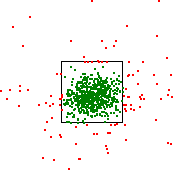
\includegraphics[width = 0.245\columnwidth ]{images/pinch.png}\label{fig:pinchHB}}} 
	\subfloat[]{\fbox{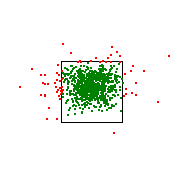
\includegraphics[width = 0.245\columnwidth ]{images/swipe.png}\label{fig:swipeHB}}}
	\subfloat[]{\fbox{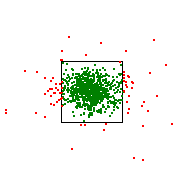
\includegraphics[width = 0.245\columnwidth ]{images/throw.png}\label{fig:throwHB}}}
	\subfloat[]{\fbox{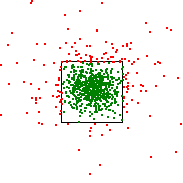
\includegraphics[width = 0.245\columnwidth ]{images/tilt.png}\label{fig:tiltHB}}}
	\caption{
		Hit location diagram for each technique. Green is a hit, red is a miss
		\protect\subref{fig:pinchHB} Pinch
		\protect\subref{fig:swipeHB} Swipe
		\protect\subref{fig:throwHB} Throw
		\protect\subref{fig:tiltHB} Tilt
	}
	\label{fig:thitboxes}
\end{figure}

\Cref{fig:thitboxes} shows that \swipe and \throw have a large concentration of hits inside the target cell, \pinch and \tilt have quite a spread of hits outside the target cell. These figures, combined with the standard deviation of the hit success of each technique, tells us that users are able to hit the targets more consistently with \swipe and \throw.

The different grid sizes also proved to be significant in regards to the accuracy of each technique. This is because regardless of which technique we are talking about, it is hard to keep the pointer completely still while performing any of the techniques. Any small movement while activating the technique might lead to the pointer leaving the cell and the user then missing the target. This effect is much more pronounced in the smaller grid size.

Looking at the survey, we can look at each question and see there is a trend.
If the user gave it a high score, then he strongly agreed with the given question.
We can then say the accumulated scores of each technique for all questions show a tendency towards the user agreeing that the given technique was easy to use.
The higher the score, the easier the user felt the given technique was to perform.
This means that in general, users considered \swipe much easier to use then the other techniques. 
\throw and \tilt were considerably close to each other, while \pinch trailed quite significantly behind.
It is interesting to note that \throw and \tilt were so close to each other in ease of use, even though \throw outperformed \tilt considerably, both in regards to time and hit success, as well as the consistency of the technique, shown by the standard deviation. 

There is though a qualitative aspect to take into account here, which is not reflected well in the surveys or the test results.
For example, a large finding was that correct mapping between the direction in which the user is point and the pointer icon on the screen is critical to the success of the application.
It is extremely important for the experience of the user to have as close to absolute mapping as possible. 
Eleven users mentioned having trouble reaching all areas of the screen, but almost all users showed sign of trouble, by for example standing on their toes or stretching their arms as far as possible.
One user got so frustrated that she asked for a chair to stand on. 
With more or different sensors, we could have had a more precise pointer by being able to determine the direction of the phone and the arm and not solely rely on the position of the users hands.
This would most likely lead to more precise results, because the the mapping between the pointer and the users pointing direction would be much closer to a absolute mapping.

In regards to the mobile phone, four users complained that the screen was too small when performing a \pinch, making it hard to precisely select the correct shape.
Four other users complained that the screen was too large when performing a swipe, since it was hard to reach the correct shape with their thumbs while still maintaining precision with the pointer. 
Four users mentioned that it was hard to orient themselves with the phone while performing the \throw technique, having to break their flow to look down on the phone to select the correct shape. 
Three users mentioned the same problem with \swipe, whenever the targets were too high.
This sometimes lead to the mobile phone covering up the target and making it hard for the user to orient themselves to the large display. 
This was an effect of the relative mapping though, since it was hard to see the screen when their arm was stretched far above their head in order to reach the high targets.
The same error could have occurred with \tilt, since the user might also end up lifting the phone in front of their field of view, but none of the users mentioned it there.  

There is also a the learning aspect of each technique. Six people actually mentioned that the \pinch technique was hard to learn, but in actuality a large portion of the participants had to be told more specifically how to perform it. 
The same held true for the \throw technique, a large number of the participants had to be told that they had to perform a slightly larger motion in order for the application to understand that a throw motion was being attempted.
Very few of the participants had to have further instructions on how the \swipe technique worked, and few people needed further help with the \tilt. 
This is most likely a combination of the complexity of some of the techniques as well as the tutorial movies not being descriptive enough. 
This also lead to frustration, were users thought they were performing the technique correctly and nothing was happening. 
Four users mentioned being frustrated by the \pinch technique, while three users got frustrated with the \tilt technique

The fatigue effect is also something to take into consideration. 13 people mentioned being fatigued through out the test and 11 of them first mentioned it during the \throw technique.
Some users commented that it was because one arm had nothing to do but be uplifted and point to the screen, while the other arm performed all the motion.
One user mentioned it would not have been that noticeable if the pointing arm had some motion to perform. 

Finally, there is also the fun aspect to take into consideration. Nine users actually mentioned having fun while performing the \pinch technique. 
They compared it to casting a spell or causing explosions on the screen. Three other users mentioned that this technique was especially interesting. 
It is still worth remembering though that \pinch was, by large, the hardest technique for users to learn. 

\subsection{Limitations}
There are of course some limitations to the system we developed. 
Firstly, the intention with the \tilt technique was that the users would point and tilt with the phone, but because of our implementation, it was possible for users to point with one hand and tilt the phone with the other.
The same holds true for the \swipe technique, where users were able to point with one hand and swipe with the other.

The way the system detects an open hand is not very robust: sometimes, depending on the profile of the hand, it misreads the users intentions and believes the user opened his hand. 

The system also has a very narrow definition of what throwing means. 
This is something that can be seen when users were told to "throw" the data from the phone to the screen.
Some would perform a much larger tilt motion, others would perform a baseball-like pitching motion. 

The Kinect also had some problems determining where the different arm joints were.
If the elbow joint was directly behind the hand joint from the Kinects perspective, it would cause the pointer to move erratically since the Kinect was not absolutely sure were the hand joint was.
Another problem occurred when the user put their two hands close to each other. 
The Kinect would have problems determining where the individual hand joints were located. 
